\documentclass[11pt]{report}
\usepackage{amsmath}
\usepackage{amsfonts}
\usepackage{amsthm}
\usepackage{ragged2e}
\usepackage{hyperref}
\usepackage{float}
\usepackage{pgf,tikz}
\usepackage[shortlabels]{enumitem}
\usepackage{color}
\usepackage{pgfplots}
\usepackage[margin = 1 in]{geometry}
\usepackage{mathrsfs}
\usetikzlibrary{arrows}
\usepackage{multicol}
\usepackage{fancyhdr}
\pagestyle{fancy}
\usepackage{multirow}
\usepackage{graphicx}
\usepackage{psfrag}
\usepackage{upgreek}
\renewcommand{\footrulewidth}{0.4pt}

\newcounter{appdef}
\setcounter{appdef}{2}
\newtheorem{theorem}{Theorem}[chapter]
\newtheorem{defn}{Definition}[appdef]
\newtheorem{lemma}{Lemma}[appdef]

\theoremstyle{definition}
\newtheorem{proposition}{Proposition}[chapter]
\newtheorem{remark}{Remark}[chapter]
\newtheorem{example}{Example}[appdef]

\newcommand{\user}{}
\newcommand{\xlr}[2]{#1 \left(#2\right)}
\newcommand{\clr}[2]{#1 \left\{ #2 \right\}}
\newcommand{\spn}{\operatorname{span}}
\lhead{ECE 515 - Fall 2019 at University of Illinois at Urbana-Champaign}
% \rhead{\textcolor{red}{HW1 - Template}}
\rhead{\textcolor{black}{HW1}}
\lfoot{Submitted by: \textcolor{red}{\textit{daweis2}}}
\rfoot{Due: \textcolor{red}{\today}}
\begin{document}

% \textcolor{red}{\textbf{Instructions:} Please edit and modify all items in red for your submission (and delete this line).}
% \newline

%==========================================================================================
\section*{Problem 1}
Consider this electrical circuit with \emph{time-varying} characteristics $R(t)$, $L(t)$ and $C(t)$. Let $q(t)$ denote the charge in capacitor at time $t$, and $\phi(t)$ be the inductor flux at time $t$. From physical laws we know:

\begin{figure}[H]
	\centering
	\vspace{1em}
	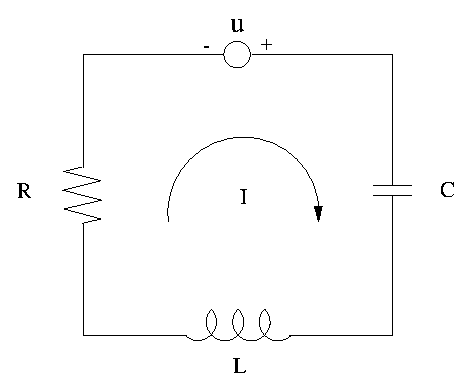
\includegraphics[trim = 0mm 0mm 0mm 20mm,height=0.9in]{circuit.eps}
\end{figure}

\begin{itemize}
\item Capacitor equation: $q(t) = C(t)V_C(t)$.
\item Inductor equation: $\phi(t)= L(t)I(t)$.
\end{itemize}
Use these laws to derive a dynamical model of this circuit which takes the form $\dot x=A(t)x+B(t)u$.

%----------------------------------------
\subsection*{Solution}
% \textcolor{red}{Type your solution here}
Let $x_1$ denote the voltage of the capacitor, and $x_2$ be the current. Then we have $\dot{q} = \dot{C}x_1 + C\dot{x_1} = x_2$ and $\dot{\phi} = \dot{L}x_2 + L\dot{x_2} = u - x_1 - x_2R$. Therefore, we have $$\dot{x_1} = \frac{-\dot{C}}{C}x_1 + \frac{1}{C}x_2,~~~\dot{x_2} = -\frac{1}{L}x_1 - \frac{R+\dot{L}}{L}x_2 + \frac{1}{L}u$$
$$A(t) = \begin{bmatrix}\frac{-\dot{C}}{C} & \frac{1}{C}\\-\frac{1}{L} & -\frac{R+\dot{L}}{L}\end{bmatrix},~~~B(t) = \begin{bmatrix}0\\\frac{1}{L}\end{bmatrix}$$.

%==========================================================================================
\section*{Problem 2}
Which of the following are vector spaces over $\mathbb{R}$ (with respect to the standard addition and scalar multiplication)? Justify your answers.

\begin{enumerate}[(a), noitemsep]
	\item The set of real-valued $n\times n$ matrices with nonnegative entries, where $n$ is a given positive integer.
	\item The set of rational functions of the form $\frac{p(s)}{q(s)}$, where $p$ and $q$ are polynomials in the complex variable $s$ and the degree of $q$ does not exceed a given fixed positive integer $k$.
	\item The space $L^2(\mathbb{R},\mathbb{R})$ of square-integrable functions, i.e., functions $f:\mathbb{R}\to\mathbb{R}$ with the property that $\int_{-\infty}^{\infty}f^2(t)dt<\infty$. ({\bf Hint: } You may use the Cauchy-Schwarz inequality, and note that this inequality applies to any inner product space.)
\end{enumerate}
%----------------------------------------
\subsection*{Solution}

% \textcolor{red}{Type your solution here}
\noindent(a) It is obvious that the $\upvartheta$ in the space must be $\theta$, an $n \times n$ matrix whose entries are all zero. However, for every matrix $M$ in the space and $M \neq \upvartheta$ there doesn't exist a matrix $\hat{M}$ so that $M + \hat{M} = \upvartheta$. Therefore this is not a vector space.

\noindent(b) This is not a vector space. For example, let $k=2$. $\frac{1}{s^2+1}$ and $\frac{1}{s+1}$ are elements in the space. However, $\frac{1}{s^2+1} + \frac{1}{s+1} = \frac{s^2+s+2}{s^3+s^2+s+2}$ is not an element in the space.

\noindent(c) The item (b)-(g) in the definition are easy to verify. We next prove that this space satisfy the constraint (a). For any $f_1 \in \mathcal{X},~f_2 \in \mathcal{X}$, we have $\int_{-\infty}^{\infty}(f_1+f_2)^2 dt = \int_{-\infty}^{\infty}f_1^2 dt + \int_{-\infty}^{\infty}f_1^2 dt + \int_{-\infty}^{\infty}f_1f_2 dt$. It's easy to verify that $\int_{-\infty}^{\infty}f_1f_2 dt$ is an inner product between $f_1$ and $f_2$ defined on $\mathcal{X}$. Therefore, according to the Cauchy-Schwarz inequality we have $\int_{-\infty}^{\infty}f_1f_2 dt \le \sqrt{\int_{-\infty}^{\infty}f_1^2 dt}\sqrt{\int_{-\infty}^{\infty}f_1^2 dt} < \infty$. Therefore, $\int_{-\infty}^{\infty}(f_1+f_2)^2 dt < \infty$ and $f_1+f_2 \in \mathcal{X}$. Therfore, this is a vector space.

%==========================================================================================
\section*{Problem 3}
A single-input, single-output linear time-invariant system is described by the transfer function:
$$ G(s) = \frac{s+4}{(s+1)(s+2)(s+3)} $$

\begin{enumerate}[(a), noitemsep]
	\item Obtain a state-space representation in controllable canonical form.
	\item Now obtain one in observable canonical form.
	\item Use the partial fraction expansion of $G(s)$ to obtain a representation of this model with a diagonal state matrix $A$.
\end{enumerate}
%----------------------------------------
\subsection*{Solution}

% \textcolor{red}{Type your solution here}

$$ G(s) = \frac{s+4}{s^3+6s^2+11s+6} $$

\noindent(a) CCF: $\dot{x} = Ax+Bu,~y=Cx$\\ where $A = \begin{bmatrix}0 & 1 & 0\\0 & 0 & 1\\-6 & -11 & -6\end{bmatrix}$; $B = \begin{bmatrix}0\\0\\1\end{bmatrix}$; $C = \begin{bmatrix}4\\1\\0\end{bmatrix}^T$.

\noindent(b) OCF: $\dot{x} = Ax+Bu,~y=Cx$\\ where $A = \begin{bmatrix}-6 & 1 & 0\\-11 & 0 & 1\\-6 & 0 & 0\end{bmatrix}$; $B = \begin{bmatrix}0\\1\\4\end{bmatrix}$; $C = \begin{bmatrix}1\\0\\0\end{bmatrix}^T$.

\noindent(c) $G(s) = \frac{3/2}{s+1} + \frac{-2}{s+2} + \frac{1/2}{s+3}$. Then we have:
$$A = \begin{bmatrix}-1 & 0 & 0\\0 & -2 & 0\\0 & 0 & -3\end{bmatrix}; B = \begin{bmatrix}\frac{3}{2}\\-2\\\frac{1}{2}\end{bmatrix}; C = \begin{bmatrix}1\\1\\1\end{bmatrix}^T; D = \begin{bmatrix}0\\0\\0\end{bmatrix}$$.


%==========================================================================================
\section*{Problem 4}
Let $A$ be the linear operator in the plane corresponding to the counter-clockwise rotation around the origin by some given angle $\theta$. Compute the matrix of $A$ relative to the standard basis in $\mathbb{R}^2$.



%----------------------------------------
\subsection*{Solution}

% \textcolor{red}{Type your solution here}
Let the bases are $e_1=[1,0]^T, e_2=[0,1]^T$, then the rotated vectors are $\hat{e_1} = [\cos\theta, \sin\theta]^T, \hat{e_2} = [-\sin\theta, \cos\theta]^T$. Because $[e_1, e_2]A = [\hat{e_1}, \hat{e_2}]$, we have $A = \begin{bmatrix}\cos\theta&-\sin\theta\\\sin\theta&\cos\theta\end{bmatrix}$.




\end{document}
